\section{Hyperparameter-Abstimmung} \label{ch:hyper_parameter_tuning}

Leider gibt es nicht für jedes Problem ein offensichtlich optimales Modell.
Ein Modell bildet den Input auf den Output ab, um jedoch zuverlässig zu bestimmen, welche Informationen in den Daten verworfen werden sollten (und somit nicht zur Generalisierung beitragen) und welche hervorgehoben werden sollten, müssen entsprechende Annahmen getroffen werden.

1996 wies David Wolpert darauf hin, dass es keinen Grund gibt, ein Modell einem anderen vorzuziehen, wenn keine Annahmen über den Datensatz getroffen werden.
Diese Argumentationslinie ist heute als \textit{No Free Lunch Theorem} bekannt \cite{Wolpert1996}.
Einige dieser Annahmen werden bereits im Vorfeld getroffen (z.B. die Verwendung von Feed-Forward-Neuronalen Netzen), andere sind jedoch Gegenstand von Optimierungen.

Die Hyperparameter-Optimierung ist ein Optimierungsproblem, bei dem der Verlust (oder andere Metriken wie z.B. die Genauigkeit) des Modells für die gegebenen Trainingsdaten minimiert werden soll.
Die im ersten Modell verwendeten Hyperparameter, die Gegenstand der Optimierung sein könnten, sind unter anderem:

\begin{enumerate}
    \item Training data:
    \begin{tasks}(2)
        \task Anzahl der Trainingsdaten
        \task Bildgröße
        \task Batch-Größe
        \task Reduzierung der Anzahl der Merkmale
    \end{tasks}
    \item Model:
    \begin{tasks}(2)
        \task Anzahl der Schichten
        \task Typen der Schichten
        \task Größe der Schichten
        \task Wahl der Verlustfunktion
    \end{tasks}
    \item Optimizer:
    \begin{tasks}(2)
        \task Wahl des Optimierers
        \task Lernrate
        \task Momentum
        \task Nesterov
    \end{tasks}
    \item Training:
    \begin{tasks}(2)
        \task Schritte pro Epoche
        \task Anzahl der Epochen
    \end{tasks}
\end{enumerate}

Einige Hyperparameter müssen getestet werden und sind nicht offensichtlich, aber andere können ohne offensichtliche negative Nebenwirkungen verbessert werden, so dass sie hier zuerst behandelt werden. Danach werden Algorithmen zum Testen verschiedener Modelle mit unterschiedlichen Hyperparametern zur Verbesserung des Modells untersucht.

\section{Augmentierung der Daten} \label{ch:data_augmentation}

Das erste, was verbessert werden kann, ist die Größe des Datensatzes, den wir für das Training des Modells verwenden.
In den vorherigen Tests sahen die Modelle jedes Bild etwa 20 Mal während des Trainings (Batches der Größe 20, 20 Schritte pro Epoche und 20 Epochen geteilt durch 400 Trainingsproben), was höchstwahrscheinlich die Ursache für die auftretende Überanpassung ist.
Die Größe des Trainingssets zu erhöhen, scheint also ein sinnvoller Ansatz zu sein.

Die Augmentierung der Daten funktioniert in diesem Fall über die Veränderung einiger Eigenschaften des Bildes, die für den jeweiligen Zweck sinnvoll sind.
Im Falle der Symbolerkennung kann das Symbol gedreht oder gespiegelt werden, so dass Trainingsbeispiele hinzugefügt werden können, ohne dass der Datenbestand redundant wird und die Daten in diesem Fall in keiner Weise weniger gültig werden.

Die Datenerweiterung wird durch Anpassung der \code{create\_generator}-Funktion durchgeführt:

\begin{lstlisting}
from tensorflow.keras.preprocessing.image import ImageDataGenerator

def create_generator(data_dir, batch_size, datagen):
    full_path = join(processed, data_dir)
    return datagen.flow_from_directory(
        full_path,
        target_size=(32, 32),
        batch_size=batch_size,
        class_mode='binary')

train_datagen = ImageDataGenerator(
        rescale = 1./255,
        rotation_range=360,
        horizontal_flip=True,
        vertical_flip=True)

test_datagen = ImageDataGenerator(rescale = 1./255)

train_generator = create_generator('train', 20, train_datagen)
test_generator = create_generator('test', 10, test_datagen)
\end{lstlisting}

Anstelle von \code{datagen = ImageDataGenerator(rescale = 1./255)} wird dieses Objekt als Parameter angegeben, da das Trainingsset zufällige Änderungen an den geladenen Daten vornimmt.
Nämlich eine zufällige Rotation und die Möglichkeit, horizontal und vertikal gespiegelt zu werden.
Bitte beachten Sie, dass keine Änderungen auf die Testdaten angewendet werden.

Die Anwendung dieser Änderungen ergibt einen Verlust von 0,61 und eine 78,75\%ige Genauigkeit der Trainingsdaten.
Der Verlust und die Genauigkeit des Testsatzes betragen 0,63 bzw. 78\%.

\begin{figure}
    \centering
    \begin{subfigure}[b]{0.4\textwidth}
        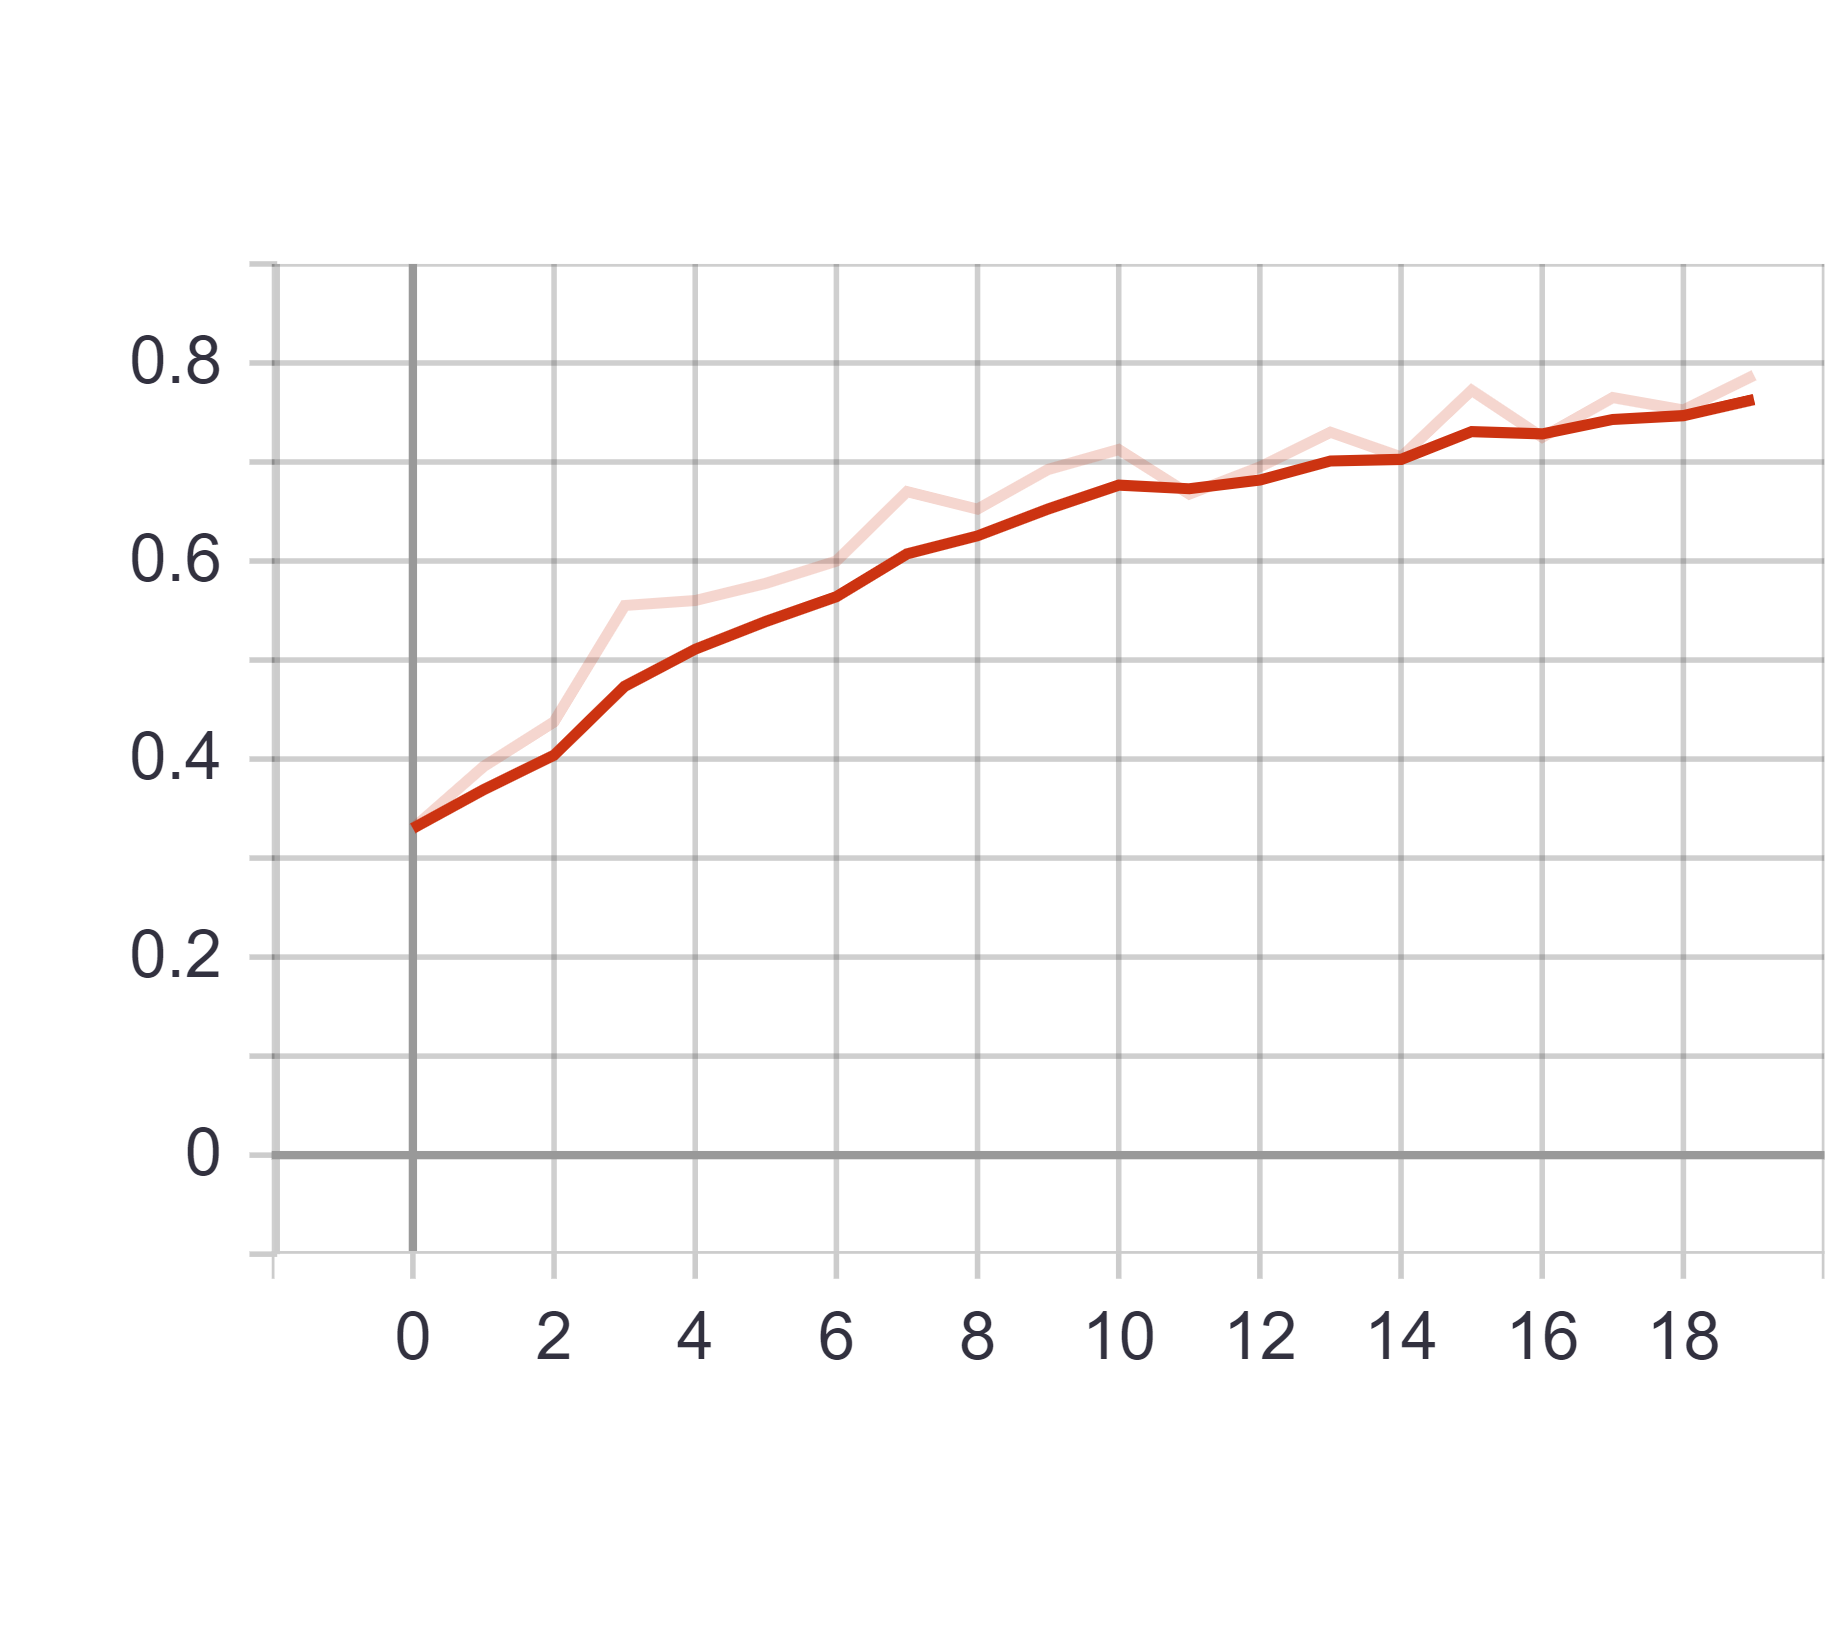
\includegraphics[width=\textwidth]{images/first_model_data_augmentation_acc.png}
        \caption{Accuracy}
        \label{fig:first_model_data_augmentation_acc}
    \end{subfigure}
    \begin{subfigure}[b]{0.4\textwidth}
        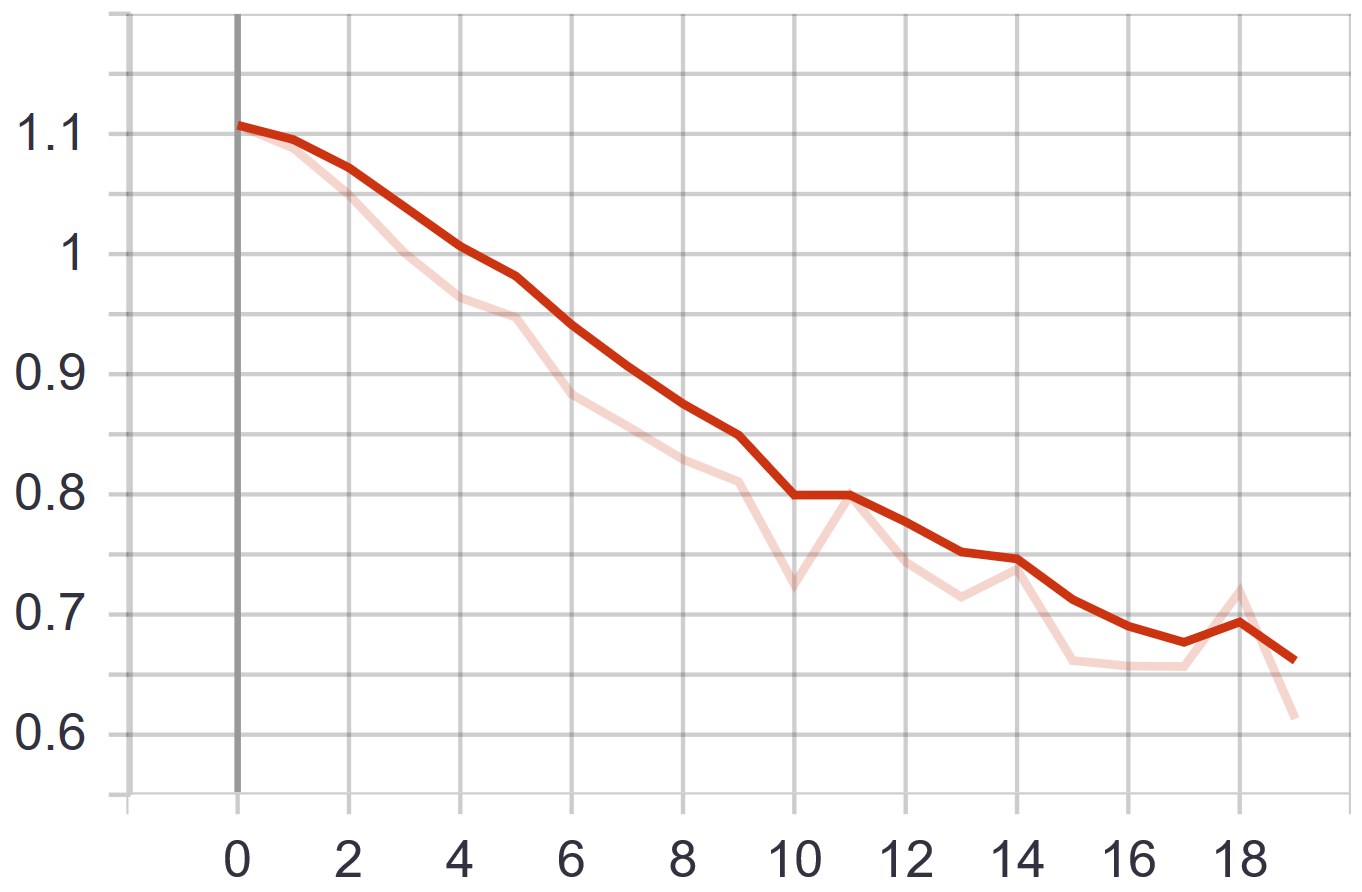
\includegraphics[width=\textwidth]{images/first_model_data_augmentation_loss.png}
        \caption{Loss}
        \label{fig:first_model_data_augmentation_loss}
    \end{subfigure}
    \caption[Training nach Augmentierung der Daten]{Im Vergleich zu Abbildung~\ref{fig:first_model_graphs} nehmen die Genauigkeit und der Verlust langsamer zu. Weitere Epochen können die Ergebnisse verbessern, da das Modell nach 20 Epochen noch nicht vollständig konvergiert zu sein scheint.}
    \label{fig:first_model_data_augmentation_graphs}
\end{figure}

Es ist offensichtlich, dass die Genauigkeit der Trainingsdaten hier tatsächlich abnimmt.
Dies ist nicht überraschend, da dem Modell keine Daten mehr zweimal gegeben werden, also keine Memorisierung stattfindet, aber da sich die Testgenauigkeit nicht geändert hat, scheint der gewünschte Effekt eingetreten zu sein.
Die Modellgenauigkeit des Trainingssatzes scheint auch mit einer geringeren Rate zu steigen, so dass mehr Epochen oder größere Batches die Performanz bereits verbessern könnten.

Bitte beachten Sie, dass das Trainingsset praktisch um den Faktor 1440 (360 Grad + Drehungen in zwei Achsen) gewachsen ist, wodurch die Möglichkeit besteht, während des Trainings wesentlich mehr Daten in das Modell einzuspeisen, ohne mit einer zu großen Überanpassung rechnen zu müssen.

Das Ziel, die Überanpassung zu verringern, scheint in dieser Hinsicht gelöst zu sein; der Unterschied zwischen Trainings- und Testgenauigkeit ist vernachlässigbar klein{\footnote{Link zum jeweiligen Notebook}: \aka{https://github.com/klawr/deepmech/blob/master/reports/srp/notebooks/6.2-feature_reduction.ipynb}}.

\subsection{Reduzierung der Merkmale}

Eine weitere Sache, die die Leistung des Modells verbessern kann, ist die Reduzierung der Größe des Inputs.
Das Phänomen, das als \textit{Fluch der Dimensionalität} bekannt ist, beschreibt die Möglichkeiten unterschiedlicher Konfigurationen, die mit zunehmender Anzahl von Variablen möglich sind, und kommt von Richard Bellman, der sich zunächst auf Probleme in der dynamischen Programmierung \cite[p.ix]{Bellman1957} bezieht.

Die Daten werden bereits stark reduziert, indem die Daten als Bilder mit einer Breite und Höhe von 32 Pixeln eingeladen werden, obwohl die Daten roh als 512 mal 512 Bilder vorliegen. Diese Reduzierung wurde im Vorfeld manuell durchgeführt, um die Daten relativ klein zu halten, die Symbole aber noch gut zu unterscheiden sind.

Obwohl die Rohdaten nur Farben in Graustufen enthalten, werden sie mit drei Farbkanälen geladen (daher die Eingabegröße \code{[32, 32, 3]}).
Eine Möglichkeit, die Eingabegröße zu reduzieren, besteht also darin, die Daten auf eine Farb-Dimension zu projizieren, wie von Géron \cite[S.215]{Geron2019} vorgeschlagen.
Der Aufruf des \code{flow\_from\_directory} wird also durch einem weiteren Parameter \code{color\_mode='grayscale'} ergänzt um den 3-dimensionalen \code{color\_mode='rgb'} (die als Standard eingestellt ist) auf eine Dimension zu reduzieren.
Praktisch sollte sich also nichts ändern, bis auf die Eingabegröße, welche auf \code{[32, 32, 1]} angepasst wird.

Das resultierende Modell sieht entsprechend folgendermaßen aus:

\begin{lstlisting}
Model: "sequential"
_________________________________________________________________
Layer (type)                 Output Shape              Param #   
=================================================================
flatten (Flatten)            (None, 1024)              0         
_________________________________________________________________
dense (Dense)                (None, 32)                32800     
_________________________________________________________________
dense_1 (Dense)              (None, 32)                1056      
_________________________________________________________________
dense_2 (Dense)              (None, 3)                 99        
=================================================================
Total params: 33,955
Trainable params: 33,955
Non-trainable params: 0
_________________________________________________________________
\end{lstlisting}

Die Anzahl der trainierbaren Parameter wird fast durch den Faktor drei geteilt und damit die Größe des Modells von 807kb (von den Vorgängermodellen mit 99491 Parametern) auf 295kb reduziert.
Hierbei geht dennoch keinerlei Genauigkeit verloren. \footnote{Link zum jeweiligen Notebook: \aka{https://github.com/klawr/deepmech/blob/master/reports/srp/notebooks/6.4-convolutional_layer.ipynb}}.

\subsection{Optimierer}

Bisher wurde nur der Optimierer des stochastischen Gradientenabstiegs betrachtet.
Der stochastische Gradientenabstieg hat mehrere Parameter, die sich optimieren lassen, z.B. die Lernrate, den Impuls und ob Nesterov verwendet wird oder nicht, wie bereits in Kapitel \ref{ch:optimizer} behandelt.

Es wurden bereits mehrere Versuche unternommen, die Suche nach diesen Hyperparametern zu automatisieren.
In diesem Projekt werden einige alternative Optimierer untersucht, aber nicht allzu ausführlich erläutert.
Bitte beachten Sie die angegebenen Quellen für weitere Einblicke.

Beim stochastischen Gradientenabstieg ist die Lernrate für alle Parameter jeder Ebene des Modells gleich.
Eine Anpassung für jeden Parameter oder sogar für einzelne Dimensionen der Schichten kann hilfreich sein, aber dies manuell zu tun würde einen unverhältnismäßig hohen Aufwand erfordern.

\name{AdaGrad} \cite{Duchi2010} ändert die Lernrate für jeden Parameter.
Dies geschieht durch Anpassung der Lernrate (beginnend mit einem einheitlichen Wert) für jeden einzelnen Parameter unter Verwendung der Größe des Gradienten für den jeweiligen Parameter.
Während dieser Ansatz bei einigen Problemen gut funktioniert, ist er bei einigen Problemen auch nicht sinnvoll.
Dennoch dient er als Grundlage für viele andere Optimierer, die nach diesem entwickelt wurden, von denen drei in dem in diesem Projekt verwendeten Tuning-Algorithmus getestet wurden.

\name{AdaDelta} \cite{Zeiler2012} ist ein modifizierter Algorithmus auf der Basis von \name{AdaGrad}, der versucht, AdaGrads Idee, die Lernrate konstant zu reduzieren, dadurch zu lösen, dass die Lernrate wieder durch einen exponentiell abklingenden Durchschnitt der Gradienten geteilt wird.
Dies führt zu einem wesentlich stabileren Optimierer, der in der Praxis gut zu funktionieren verspricht.

\name{RMSProp} \cite{Hinton2012} funktioniert ähnlich wie \name{AdaDelta} mit einer leicht abweichenden Aktualisierungsregel.
Es wird als "im Allgemeinen eine ausreichend gute Wahl, was auch immer Ihr Problem ist" \cite[S.77]{Chollet2017} betrachtet.

Adam \cite{Kingma2014}\cite{Reddi2018} ist der letzte in diesem Projekt enthaltene Optimierer, der eine weitere Methode zur Anwendung einer adaptiven Lernrate für jeden Parameter darstellt.
Adam integriert die zuvor erwähnte Idee des Impulses in einen Algorithmus, der dem von \name{RMSProp} ähnlich ist.

Es gibt weitere erwähnenswerte Optimierer (nämlich AdaMax oder Nadam), die möglicherweise Gegenstand weiterer Untersuchungen sind.

Bemerkenswert ist, dass die hier erläuterten adaptiven Methoden möglicherweise nicht bei jedem Modell funktionieren, so dass es sich immer lohnt, den zugrundeliegenden Gradientenabstieg mit Nesterov\cite[S.358]{Geron2019} zu versuchen.

\subsection{Convolutional Layers}

"Convolutional Layers" sind für die Bilderkennung weit verbreitet und es ist daher sinnvoll, sie in dieses Modell zu integrieren.
Sie wurden von Yann LeCun 1998 in einer Arbeit \cite{Lecun1998} eingeführt, um handgeschriebene Ziffern zu erkennen.

In diesem Projekt werden nur zweidimensionale "Convolutional Layers" verwendet, da die Eingabe zweidimensional ist (nachdem die Bilder in Graustufen übertragen wurden).
Der Unterschied der "Convolutional Layers" zu den zuvor beschriebenen "Dense Layers" besteht darin, dass die trainierten Parameter nicht die Verbindungen aller Knoten der vorherigen Schicht zu einer nächsten darstellen, sondern einen Kernel, der über die Eingangsschicht gleitet und als Filter fungiert, der die Ausgangsschicht aufbaut.
Dies bedeutet auch, dass die Eingangsschicht nicht flach gemacht werden muss, bevor sie in das Modell eingespeist wird.

Beim Training eines "Convolutional Layers" sind die trainierten Parameter die Filter, die eine vorgegebene Form haben.
Eine zweidimensionales "Convolutional Layer" mit acht Filtern, einer Eingabetiefe von eins und einer Kernelgröße von vier mal vier (und einer für den Bias) hat 136 (8 x (1 x 4 x 4 + 1)) Parameter zu trainieren, was deutlich weniger als bei früheren Ansätzen ist und nicht von der Größe der Eingangsschicht abhängt, so dass es möglich ist, Muster in beliebig großen Bildern zu erkennen, ohne dass das Modell selber vergrößert werden muss.

Die entsprechende Gleichung für eine einzelne Aktivierung ist daher durch \cite[S. 453]{Geron2019} gegeben:
\begin{equation}
    z_{i,j,k} = b_k + \sum_{u=1}^{h} \sum_{v=1}^{w} \sum_{k'=1}^{n'} x_{i', j', k'} \times w_{u, v, k', k} 
\end{equation}

Dabei ist $z$ der Aktivierungswert, wobei die Indizes $i$ und $j$ die Position des Knotens in der Ausgabeschicht und $k$ den Index des Filters darstellen.
Die Summe aller Eingabeknoten ergibt sich aus der Summe der Knoten in den jeweiligen Richtungen, die durch Iteration über drei Achsen unter Verwendung der Höhe ($h$), der Breite ($w$) und der Filtergröße ($n'$) der vorhergehenden Ebene gegeben ist.
Für jede dieser Kombinationen wird das jeweilige Verbindungsgewicht $w_{u, v, k', k}$ mit der Eingabe $x_{i', j', k'}$ an der jeweiligen Position in der vorhergehenden Schicht multipliziert, wobei $i' = i \-mal s_h + u$ bzw. $j' = j \-mal s_w$ ist und $s_h$ und $s_w$ die Schritte sind, die bei jedem Schritt in jede Richtung unternommen werden. Die Schritte reduzieren dabei die Größe der nachfolgenden Schicht.
Zusätzlich hat jeder Filter seinen eigenen Bias $b_k$, der zur Aktivierungsfunktion hinzugefügt wird.

\begin{figure}
    \centering
    \caption[Konvolutionelle Ebene]{  Die unterste Ebene ist die Eingabe, die durch eine zweidimensionale Ebene in der Größe von fünf mal fünf (Filtergröße ist eins) repräsentiert wird, die mit einem Padding von eins (grau gezeichnet) versehen ist, um sicherzustellen, dass die Größe bei Verwendung eines Kernels der Größe drei mal drei (hervorgehoben durch die roten, grünen und blauen Rechtecke) gleich bleibt. Der verwendete Stride ist eins, d.h. das rezeptive Feld propagiert bei jedem Schritt einen Eingangsknoten. Hier beginnt der Prozess am roten Rechteck, blau ist der zweite Schritt und grün der letzte (insgesamt 25 Schritte). }
    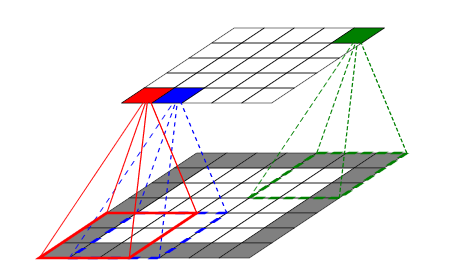
\includegraphics[width=0.6\textwidth]{images/conv_layer.png}
    \label{fig:conv_layer}
\end{figure}

Damit die Ausgabe die gleiche Größe wie die Eingabe hat, müssen Zahlen zur Eingabe addiert werden, da ein Kernel, der in jeder Richtung größer als eins ist, eine Kante für die Eingabe nicht überqueren kann (und der Schritt 1 mal 1 sein muss).
Daher wird das Padding zur Lösung dieses Problems verwendet, indem man (typischerweise) Nullen um die Eingabe herum anfügt, was zu einer Technik führt, die man Zero-Padding nennt.

Durch die Verwendung von "Convolutional Layers" anstelle von "Dense Layers" wird die Modellgröße weiter reduziert (295kb bis 232kb) und die Genauigkeit um einige Prozente erhöht. Durch das Hinzufügen von Pooling wird die Größe weiter auf 149kb reduziert und die Genauigkeit wird weiter verbessert\footnote{Verknüpfung mit den jeweiligen Notebooks: \aka{https://github.com/klawr/deepmech/blob/master/reports/srp/notebooks/6.4-convolutional_layer.ipynb} und \aka{https://github.com/klawr/deepmech/blob/master/reports/srp/notebooks/6.4.1-convolutional_layer_pooling.ipynb}}.
Pooling ist eine Technik, bei der ein Kernel (ähnlich wie der Kern von "Convolutional Layers") über die Eingabeschicht scannt.
Im verknüpften Notizbuch wurde ein Kernel paarweise verwendet, der den maximalen Wert des Kernels nimmt und nur den maximalen Wert weiterleitet, wodurch die Ausgabegröße in Breite und Höhe halbiert wird\footnote{Dies wird passenderweise \name{MaxPooling} genannt.}.

\subsection{Tuning Algorithmen}

Unter Berücksichtigung aller Möglichkeiten, das Modell vor dem Training zu optimieren, wurden einige Ansätze entwickelt, um die Hyperparameter automatisch zu optimieren.
Eine Möglichkeit, die Hyperparameter einzustellen, besteht darin, jeden einzelnen mit verschiedenen Werten zu testen, wobei die Werte aller anderen Hyperparameter festgesetzt werden.
Dies wird dann für alle Hyperparameter wiederholt.
Dieses Verfahren stellt sicher, dass der optimale Satz von Hyperparametern verwendet wird, kann aber eine inakzeptable Zeit in Anspruch nehmen, da die Anzahl der erstellten Modelle exponentiell mit der Anzahl der anzupassenden Hyperparameter wächst.
Bei zwei Hyperparametern wäre dies gleichbedeutend mit der Überprüfung jedes Wertes auf einem zweidimensionalen Gitter, daher heißt die Methode "grid search"\footnote{Wenn nur ein Hyperparameter angepasst wird, nennt man das Verfahren "linear search".}.

Ein weiterer, in der Praxis häufig verwendeter Ansatz ist die Zufallssuche.
Die Zufallssuche geht nach dem Prinzip, Hyperparameter nach dem Zufallsprinzip zuzuordnen und so verschiedene Modelle zu testen, ohne dass eine Kombination einen Vorteil bringt.
Natürlich führt dies (höchstwahrscheinlich) nicht zu einem optimalen Ergebnis, aber in der Praxis wird dieser Ansatz häufig verwendet, da er in der Regel ein akzeptables Ergebnis liefert, indem er ein breites Spektrum möglicher Konfigurationen prüft.
Ein Notizbuch wurde erstellt, um die Implementierung von \name{keras tuner} in diesem Projekt unter \aka{https://github.com/klawr/deepmech/blob/master/reports/srp/notebooks/6.5.2-random_tuner.ipynb} zu zeigen.

Einige ausgefeiltere Methoden basieren auf dem Ansatz der Zufallssuche, bei dem die Ergebnisse der Zufallssuche wiederholt untersucht werden und dann die Hyperparameter zugunsten derjenigen abgestimmt werden, die bessere Modelle zu ergeben versprechen.
Dieser Ansatz wird als Zoomen bezeichnet, da man nach jeder Iteration in den vielversprechendsten Bereich der Hyperparameter "hineinzoomen" kann.

Andere Ansätze versuchen, diesen Prozess vollständig zu automatisieren.
Beliebte Algorithmen basieren auf der Bayes'schen Optimierung, aber diese werden in diesem Projekt nicht behandelt und daher ausgelassen.

Der in diesem Projekt verwendete Tuner heißt \name{Hyperband} \cite{Li2018}, der in der Bibliothek \name{keras-tuner} implementiert wird \cite{Google2019a}.
Im Wesentlichen trainiert \name{Hyperband} Modelle mittels Zufallssuche, schränkt aber das Training für ein breites Spektrum von Hyperparametern in einigen wenigen Epochen ein.
Dies geschieht indem die Modelle für einige Epochen trainiert werden und nur die vielversprechendsten Modelle für weitere Iterationen behalten werden.
Diese Methode verspricht eine wesentlich bessere Nutzung der Ressourcen und wird mit hoher Wahrscheinlichkeit gute Hyperparameter präsentieren können.

Der endgültige Modell-Tuner ist so konzipiert, dass er ein \code{Hyperparameter}-Objekt akzeptiert, das einer Funktion zugeführt wird, die das jeweilige Modell zurückgibt:


% TODO python
\begin{lstlisting}
def create_model(hp):
    model = models.Sequential()
    model.add(layers.Conv2D(2**hp.Int('2**num_filter_0', 4, 6),
        (4,4) ,activation='relu', input_shape=(32, 32, 1)))

    for i in range(hp.Int('num_cnn_layers', 0, 3)):
        filter = 2**hp.Int('2**num_filter_' + str(i), 4, 7)
        model.add(
            layers.Conv2D(filter, (4,4), activation='relu',padding='same'))
        if hp.Boolean('pooling_' + str(i)):
            model.add(layers.MaxPooling2D(2, 2))

    model.add(layers.Flatten())
    for i in range(hp.Int('num_dense_layers', 1, 3)):
        nodes = 2**hp.Int('2**num_nodes_' + str(i), 4, 7)
        model.add(layers.Dense(nodes, activation='relu'))
    
    model.add(layers.Dense(3, 'softmax'))

    optimizers = {
        'adam': Adam(),
        'sgd': SGD(lr=hp.Choice(
            'learning_rate', [0.001, 0.003, 0.007, 0.01 0.03]),
            momentum=hp.Float('momentum', 0.6, 1, 0.1),
            nesterov=hp.Boolean('nesterov')),
        'rms': RMSprop(lr=hp.Choice(
            'learning_rate', [0.001, 0.003, 0.007,0.01, 0.03]))
    }

    model.compile(
        loss='sparse_categorical_crossentropy',
        optimizer=optimizers[hp.Choice('optimizer', list(optimizers.keys()),
        metrics=['acc'])

    return model
\end{lstlisting}

Diese Funktion erweitert \ref{lst:first_model} durch die Implementierung von Hyperparametern unter Verwendung des \code{Hyperparameter} von \name{keras tuner}.
Dies wird später mit Hilfe einer benutzerdefinierten Klasse implementiert \footnote{Die Ergebnisse wurden mit \name{TensorBoard} protokolliert, dessen API von \name{keras tuner} selbst noch nicht unterstützt wird, daher wird der Tuner von einer benutzerdefinierten Klasse vererbt}:

\begin{lstlisting}
tuner = customTuner(
    create_model,
    hyperparameters=hp,
    objective='acc',
    max_trials=100,
    executions_per_trial=1,
    directory=log_dir,
    project_name=timestamp)
\end{lstlisting}

Das Training, das vorher durch die \code{fit}-Funktion durchgeführt wurde, wird nun durch die \code{search}-Funktion des Tuners durchgeführt:

\begin{lstlisting}
tuner.search(
    train_dataset,
    validation_data=validation_dataset,
    epochs=30,
    steps_per_epoch=100,
    validation_steps=100,
    verbose=0,
    callbacks=callbacks)
\end{lstlisting}

Ein weiterer Hinweis, der hier zu beachten ist, ist, dass die in \ref{ch:data_augmentation} verwendeten Generatoren durch eine manuelle Augmentierung der Daten und spätere Vorverarbeitung unter Verwendung von Protokollbuffern(\name{protobufs}) ersetzt wurden\footnote{Das endgültige Notizbuch, das diese verwendet, kann unter \aka{https://github.com/klawr/deepmech/blob/master/reports/srp/notebooks/6.5.1-manual_data_augmentation.ipynb} eingesehen werden}.
Durch die Vorverarbeitung der Bilddaten im Vorfeld wird die Ladezeit der Daten deutlich reduziert.
Der dafür verwendete Code kann hier eingesehen werden: \aka{https://github.com/klawr/deepmech/blob/master/reports/srp/notebooks/6.5.3-hyperband.ipynb}.

Nach der Überprüfung der Daten konnte eine Genauigkeit von 96,7\% auf die Testdaten bei einer Modellgröße von 4,3mb erreicht werden.

\subsection{Vergrößerung des Trainingssets}

Nachdem das Modell angepasst wurde, wurde noch ein anderer Ansatz versucht, um die Genauigkeit zu erhöhen.
Die rohen Trainingsdaten wurden mehr als verdreifacht (auf 1000 Beispiele für jedes Symbol in den Trainingsdaten) und dann mit 32 Wiederholungen erweitert, was zu einem Datensatz von 96000 verschiedenen Bildern führte.

Bei Verwendung dieses Datensatzes wurde bei fast jedem zuvor getesteten Modell eine Genauigkeit von über 99\% erreicht.
Diese Situation präsentiert die Minimierung des Modells als wichtigstes Optimierungsziel.
Das endgültige Modell wird manuell reduziert und abgestimmt, indem Schichten und Hyperparameter reduziert werden.
Das endgültige Modell hat eine Größe von 207kb mit einer Genauigkeit von 99,3\% und einem Verlust von 0.04 auf das Trainingsset, was zufriedenstellende Ergebnisse darstellt.

Das Modell wird zusammengefasst als:

\begin{lstlisting}
model = models.Sequential()
model.add(layers.Conv2D(16, (4,4), activation='relu', padding='same',
    input_shape=(32, 32, 1)))
model.add(layers.MaxPooling2D(2,2))
model.add(layers.Conv2D(32, (4,4), activation='relu', padding='same'))
model.add(layers.MaxPooling2D(2,2))
model.add(layers.Flatten())
model.add(layers.Dense(3, 'softmax'))

optimizer = Adam()
model.compile(loss='sparse_categorical_crossentropy',
    optimizer=optimizer,metrics=['acc'])
\end{lstlisting}

Der endgültige Code für die Modellerstellung kann unter \aka{https://github.com/klawr/deepmech/blob/master/src/models/symbol_classifier.py} eingesehen werden.
